%%%%%%%%%%%%%%
%% Run LaTeX on this file several times to get Table of Contents,
%% cross-references, and citations.

%% w-bktmpl.tex. Current Version: Feb 16, 2012
%%%%%%%%%%%%%%%%%%%%%%%%%%%%%%%%%%%%%%%%%%%%%%%%%%%%%%%%%%%%%%%%
%
%  Template file for
%  Wiley Book Style, Design No.: SD 001B, 7x10
%  Wiley Book Style, Design No.: SD 004B, 6x9
%
%  Prepared by Amy Hendrickson, TeXnology Inc.
%  http://www.texnology.com
%%%%%%%%%%%%%%%%%%%%%%%%%%%%%%%%%%%%%%%%%%%%%%%%%%%%%%%%%%%%%%%%

%%%%%%%%%%%%%%%%%%%%%%%%%%%%%%%%%%%%%%%%%%%%%%%%%%%%%%%%%%%%%%%%
%% Class File

%% For default 7 x 10 trim size:
%\documentclass{WileySev}

%% Or, for 6 x 9 trim size
\documentclass{WileySix}

%%%%%%%%%%%%%%%%%%%%%%%%%%%%%%%%%%%%%%%%%%%%%%%%%%%%%%%%%%%%%%%%
%% Post Script Font File

% For PostScript text
% If you have font problems, you may edit the w-bookps.sty file
% to customize the font names to match those on your system.

\usepackage{w-bookps}

%%%%%%%
%% For times math: However, this package disables bold math (!)
%% \mathbf{x} will still work, but you will not have bold math
%% in section heads or chapter titles. If you don't use math
%% in those environments, mathptmx might be a good choice.

% \usepackage{mathptmx}


%%%%%%%%%%%%%%%%%%%%%%%%%%%%%%%%%%%%%%%%%%%%%%%%%%%%%%%%%%%%%%%%
%% Graphicx.sty for Including PostScript .eps files

\usepackage{graphicx}


%%%%%%%%%%%%%%%%%%%%%%%%%%%%%%%%%%%%%%%%%%%%%%%%%%%%%%%%%%%%%%%%
%% Other packages you might want to use:

% for chapter bibliography made with BibTeX
% \usepackage{chapterbib}

% for multiple indices
% \usepackage{multind}

% for answers to problems
% \usepackage{answers}




%%%%%%%%%%%%%%%%%%%%%%%%%%%%%%%%%%%%%%%%%%%%%%%%%%%%%%%%%%%%%%%%
%% Change options here if you want:
%%
%% How many levels of section head would you like numbered?
%% 0= no section numbers, 1= section, 2= subsection, 3= subsubsection
%%==>>
\setcounter{secnumdepth}{3}

%% How many levels of section head would you like to appear in the
%% Table of Contents?
%% 0= chapter titles, 1= section titles, 2= subsection titles, 
%% 3= subsubsection titles.
%%==>>
\setcounter{tocdepth}{2}

%% Cropmarks? good for final page makeup
%% \docropmarks %% turn cropmarks on

%%%%%%%%%%%%%%%%%%%%%%%%%%%%%%%%%%%%%%%%%%%%%%%%%%%%%%%%%%%%%%%%
%% DRAFT
%
% Uncomment to get double spacing between lines, current date and time
% printed at bottom of page.
% \draft
% (If you want to keep tables from becoming double spaced also uncomment
% this):
% \renewcommand{\arraystretch}{0.6}
%%%%%%%%%%%%%%%%%%%%%%%%%%%%%%

\begin{document}

%%%%%%%%%%%%%%%%%%%%%%%%%%%%%%%%%%%%%%%%%%%%%%%%%%%%%%%%%%%%%%%%
%% Title Pages
%%
%% Wiley will provide title and copyright page, but you can make
%% your own titlepages if you'd like anyway

%% Setting up title pages, type in the appropriate names here:
\booktitle{Sistem Informasi Geografis}
\subtitle{Mengenal dan Membangun SIG}

\author{Rolly Maulana Awangga}
%\affil{Program Studi Sarjana Terapan Teknik Informatika Politeknik Pos Indonesia}
%or
%\authors{}

%% \\ will start a new line.
%% You may add \affil{} for affiliation, ie,
%\authors{Robert M. Groves\\
%\affil{Universitat de les Illes Balears}
%Floyd J. Fowler, Jr.\\
%\affil{University of New Mexico}
%}

%% Print Half Title and Title Page:
\halftitlepage
\titlepage


%%%%%%%%%%%%%%%%%%%%%%%%%%%%%%%%%%%%%%%%%%%%%%%%%%%%%%%%%%%%%%%%
%% Off Print Info

%% Add your info here:
\offprintinfo{Sistem Informasi Geografis, pre-release}{Rolly Maulana Awangga}

%% Can use \\ if title, and edition are too wide, ie,
%% \offprintinfo{Survey Methodology,\\ Second Edition}{Robert M. Groves}


%%%%%%%%%%%%%%%%%%%%%%%%%%%%%%%%%%%%%%%%%%%%%%%%%%%%%%%%%%%%%%%%
%% Copyright Page

\begin{copyrightpage}{2017}
Sistem Informasi Geografis / Rolly Maulana Awangga
\end{copyrightpage}

% Note, you must use \ to start indented lines, ie,
% 
% \begin{copyrightpage}{2004}
% Survey Methodology / Robert M. Groves . . . [et al.].
% \       p. cm.---(Wiley series in survey methodology)
% \    ``Wiley-Interscience."
% \    Includes bibliographical references and index.
% \    ISBN 0-471-48348-6 (pbk.)
% \    1. Surveys---Methodology.  2. Social 
% \  sciences---Research---Statistical methods.  I. Groves, Robert M.  II. %
% Series.\\

% HA31.2.S873 2004
% 001.4'33---dc22                                             2004044064
% \end{copyrightpage}

%%%%%%%%%%%%%%%%%%%%%%%%%%%%%%%%%%%%%%%%%%%%%%%%%%%%%%%%%%%%%%%%
%% Frontmatter >>>>>>>>>>>>>>>>

%%%%%%%%%%%%%%%%%%%%%%%%%%%%%%%%%%%%%%%%%%%%%%%%%%%%%%%%%%%%%%%%
%% Only Dedication (optional) 
%% or Contributor Page for edited books
%% before \tableofcontents

\dedication{For my family}

% ie,
%\dedication{To my parents}

%%%%%%%%%%%%%%%%%%%%%%%%%%%%%%%%%%%%%%%%%%%%%%%%%%%%%%%%%%%%%%%%
%  Contributors Page for Edited Book
%%%%%%%%%%%%%%%%%%%%%%%%%%%%%%%%%%%%%%%%%%%%%%%%%%%%%%%%%%%%%%%%

% If your book has chapters written by different authors,
% you'll need a Contributors page.

% Use \begin{contributors}...\end{contributors} and
% then enter each author with the \name{} command, followed
% by the affiliation information.

% \begin{contributors}
% \name{Masayki Abe,} Fujitsu Laboratories Ltd., Fujitsu Limited, Atsugi,
% Japan

% \name{L. A. Akers,} Center for Solid State Electronics Research, Arizona
% State University, Tempe, Arizona

% \name{G. H. Bernstein,} Department of Electrical and
% Computer Engineering, University of Notre Dame, Notre Dame, South Bend, 
% Indiana; formerly of
% Center for Solid State Electronics Research, Arizona
% State University, Tempe, Arizona 
% \end{contributors}

%%%%%%%%%%%%%%%%%%%%%%%%%%%%%%%%%%%%%%%%%%%%%%%%%%%%%%%%%%%%%%%%
\contentsinbrief %optional
\tableofcontents
% \listoffigures %optional
% \listoftables  %optional

%%%%%%%%%%%%%%%%%%%%%%%%%%%%%%%%%%%%%%%%%%%%%%%%%%%%%%%%%%%%%%%%
% Optional Foreword:

%\begin{foreword}
%text
%\end{foreword}

%%%%%%%%%%%%%%%%%%%%%%%%%%%%%%%%%%%%%%%%%%%%%%%%%%%%%%%%%%%%%%%%
% Optional Preface:

%\begin{preface}
% text
%\prefaceauthor{}
%\where{place\\
% date}
%\end{preface}

% ie,
% \begin{preface}
% This is an example preface.
% \prefaceauthor{R. K. Watts}
% \where{Durham, North Carolina\\
% September, 2004}

%%%%%%%%%%%%%%%%%%%%%%%%%%%%%%%%%%%%%%%%%%%%%%%%%%%%%%%%%%%%%%%%
% Optional Acknowledgments:

% \acknowledgments
% acknowledgment text
% \authorinitials{} % ie, I. R. S.


%%%%%%%%%%%%%%%%%%%%%%%%%%%%%%%%
%% Glossary Type of Environment:

% \begin{glossary}
% \term{<term>}{<description>}
% \end{glossary}

%%%%%%%%%%%%%%%%%%%%%%%%%%%%%%%%
% \begin{acronyms} 
% \acro{<term>}{<description>}
% \end{acronyms}

%%%%%%%%%%%%%%%%%%%%%%%%%%%%%%%%
%% In symbols environment <term> is expected to be in math mode; 
%% if not in math mode, use \term{\hbox{<term>}}

% \begin{symbols}
% \term{<math term>}{<description>}
% \term{\hbox{<non math term>}}Box used when not using a math symbol.
% \end{symbols}

%%%%%%%%%%%%%%%%%%%%%%%%%%%%%%%%
% \begin{introduction}
%\introauthor{<name>}{<affil>}
% Introduction text...
% \end{introduction}

%%%%%%%%%%%%%%%%%%%%%%%%%%%%%%%%%%%%%%%%%%%%%%%%%%%%%%%%%%%%%%%%
%% End for Front Matter, Beginning of text of book  >>>>>>>>>>>

%% Short version of title without \\ may be written in sq. brackets:

%% Optional Part :
\part[Pengolahan Data Geospasial]
{Pengolahan Data\\ Geospasial}

\chapter[Pendahuluan]
{Pengantar\\ Sistem Informasi Geografis}
\prologue{The sheer volumne of answers can often stifle insight...The purpose
of computing\index{computing!the purpose} is insight, not numbers.}
{Hamming}

\section{Definisi}
Sistem Informasi Geografis merupakan penggalan kata dan Sistem Informasi dan Geografis. Geografis dipandang sebagai bentukan dari geospasial.
Geospasial memiliki arti geo yang berarti bumi dan spasial yang berarti ruang atau keruangan. Jadi geospasial merupakan ilmu yang mempelajari 
tata ruang dari bumi. Tata ruang melingkupi letak suatu titik di bumi baik itu letak kota, provinsi atau negara. Tata ruang juga menyajikan gambaran dari ruang tersebut yang disebut dengan ilmu kartografi atau sering disebut sebagai ilmu pembuatan peta\cite{IEEEhowto:IEEEtranpage}.

\section{Sejarah Peta}
Perkembangan peta dunia tidak luput dari para ahli geografi dan kartografi. Peta dunia yang populer pada saat ini merupkan kontribusi dari para 
pembuat peta sebelumnya

\subsection{Ptolemy's}
Ptolemy's diduga membuat peta pada abad ke 2


\subsection{Muhammad al-Idrisi}
Seorang ahli geografi dan kartografi Muhammad al-Idrisi membuat peta dunia pada abad ke 11

\begin{figure}[ht]

\centerline{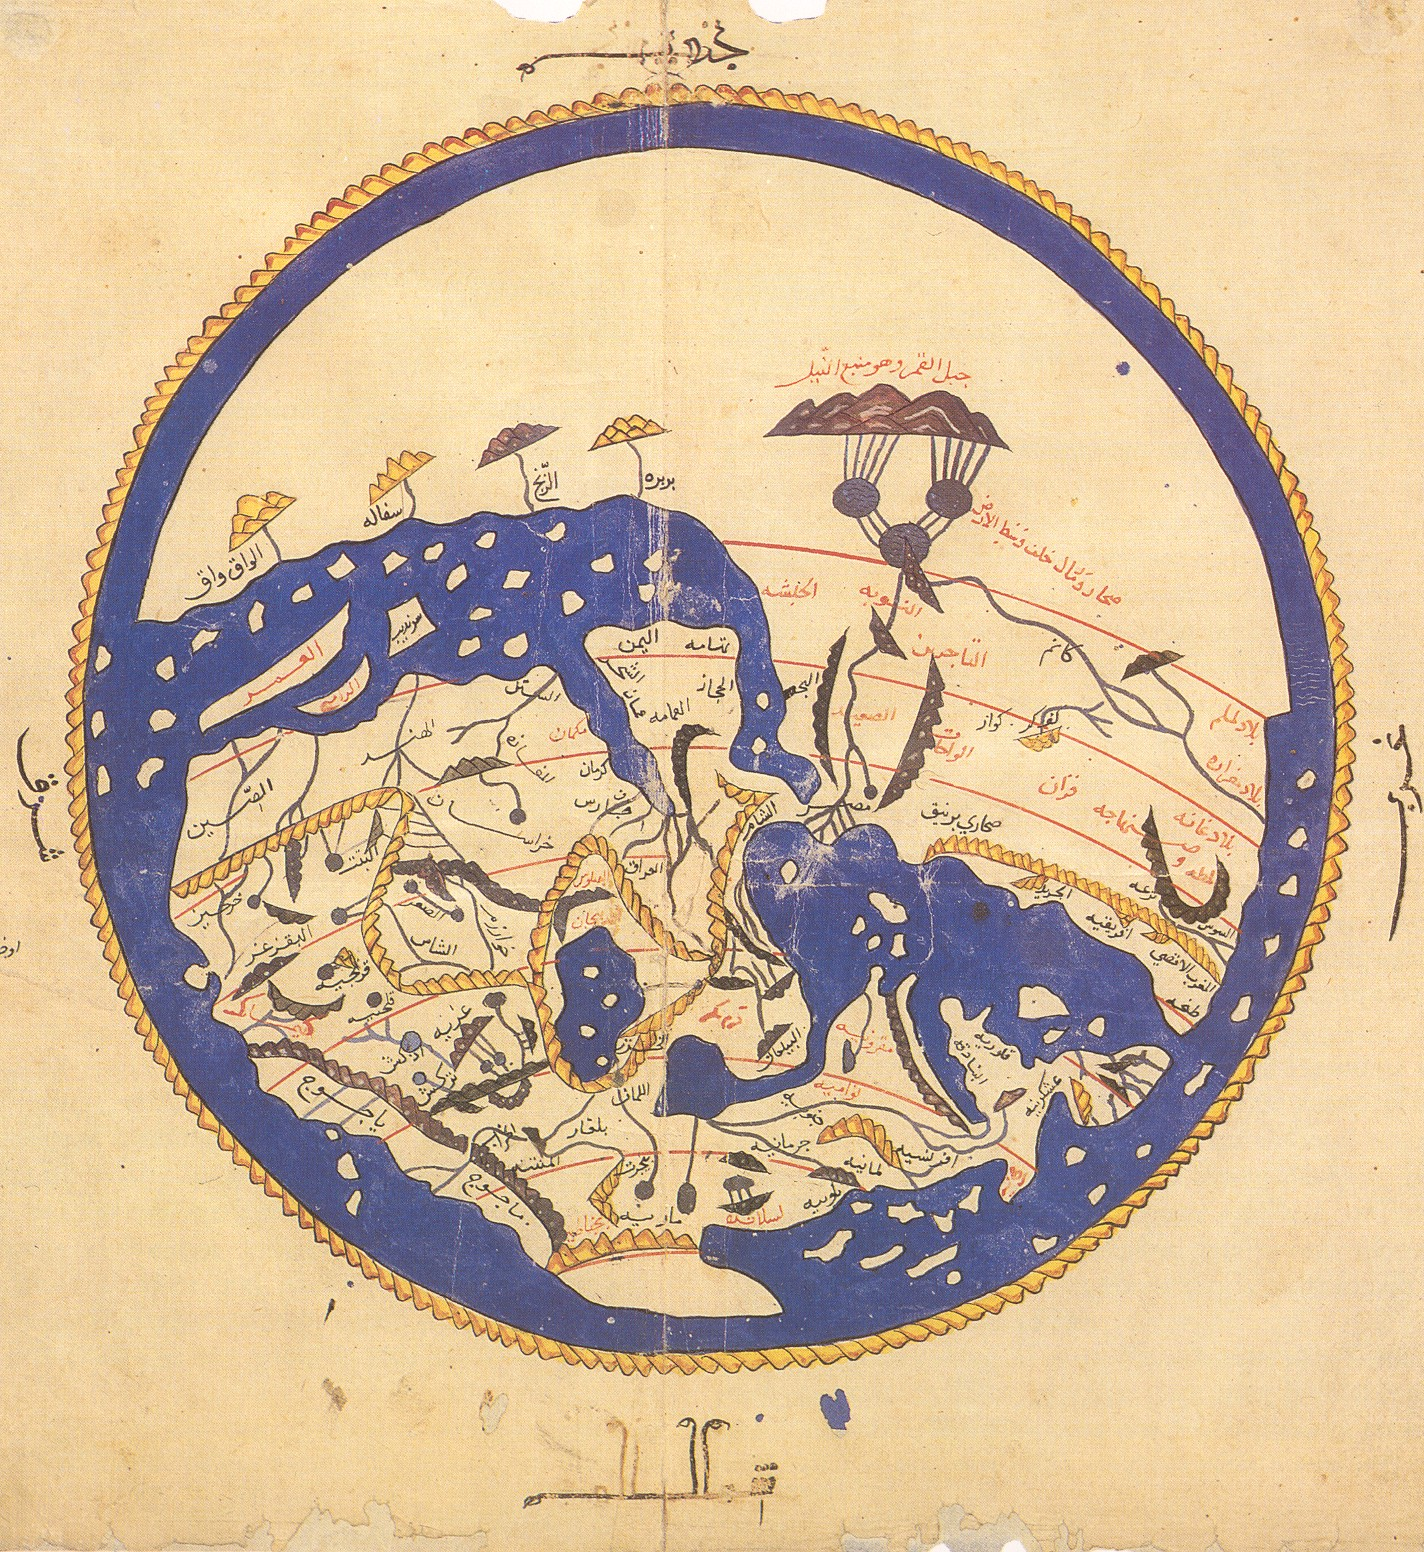
\includegraphics[width=1\textwidth]{figures/petaduniaalid.JPG}}
\caption{Gambaran pengantar peta dunia karya al-Idrisi tahun 1154.}
\end{figure}

\begin{figure}[ht]
	\centerline{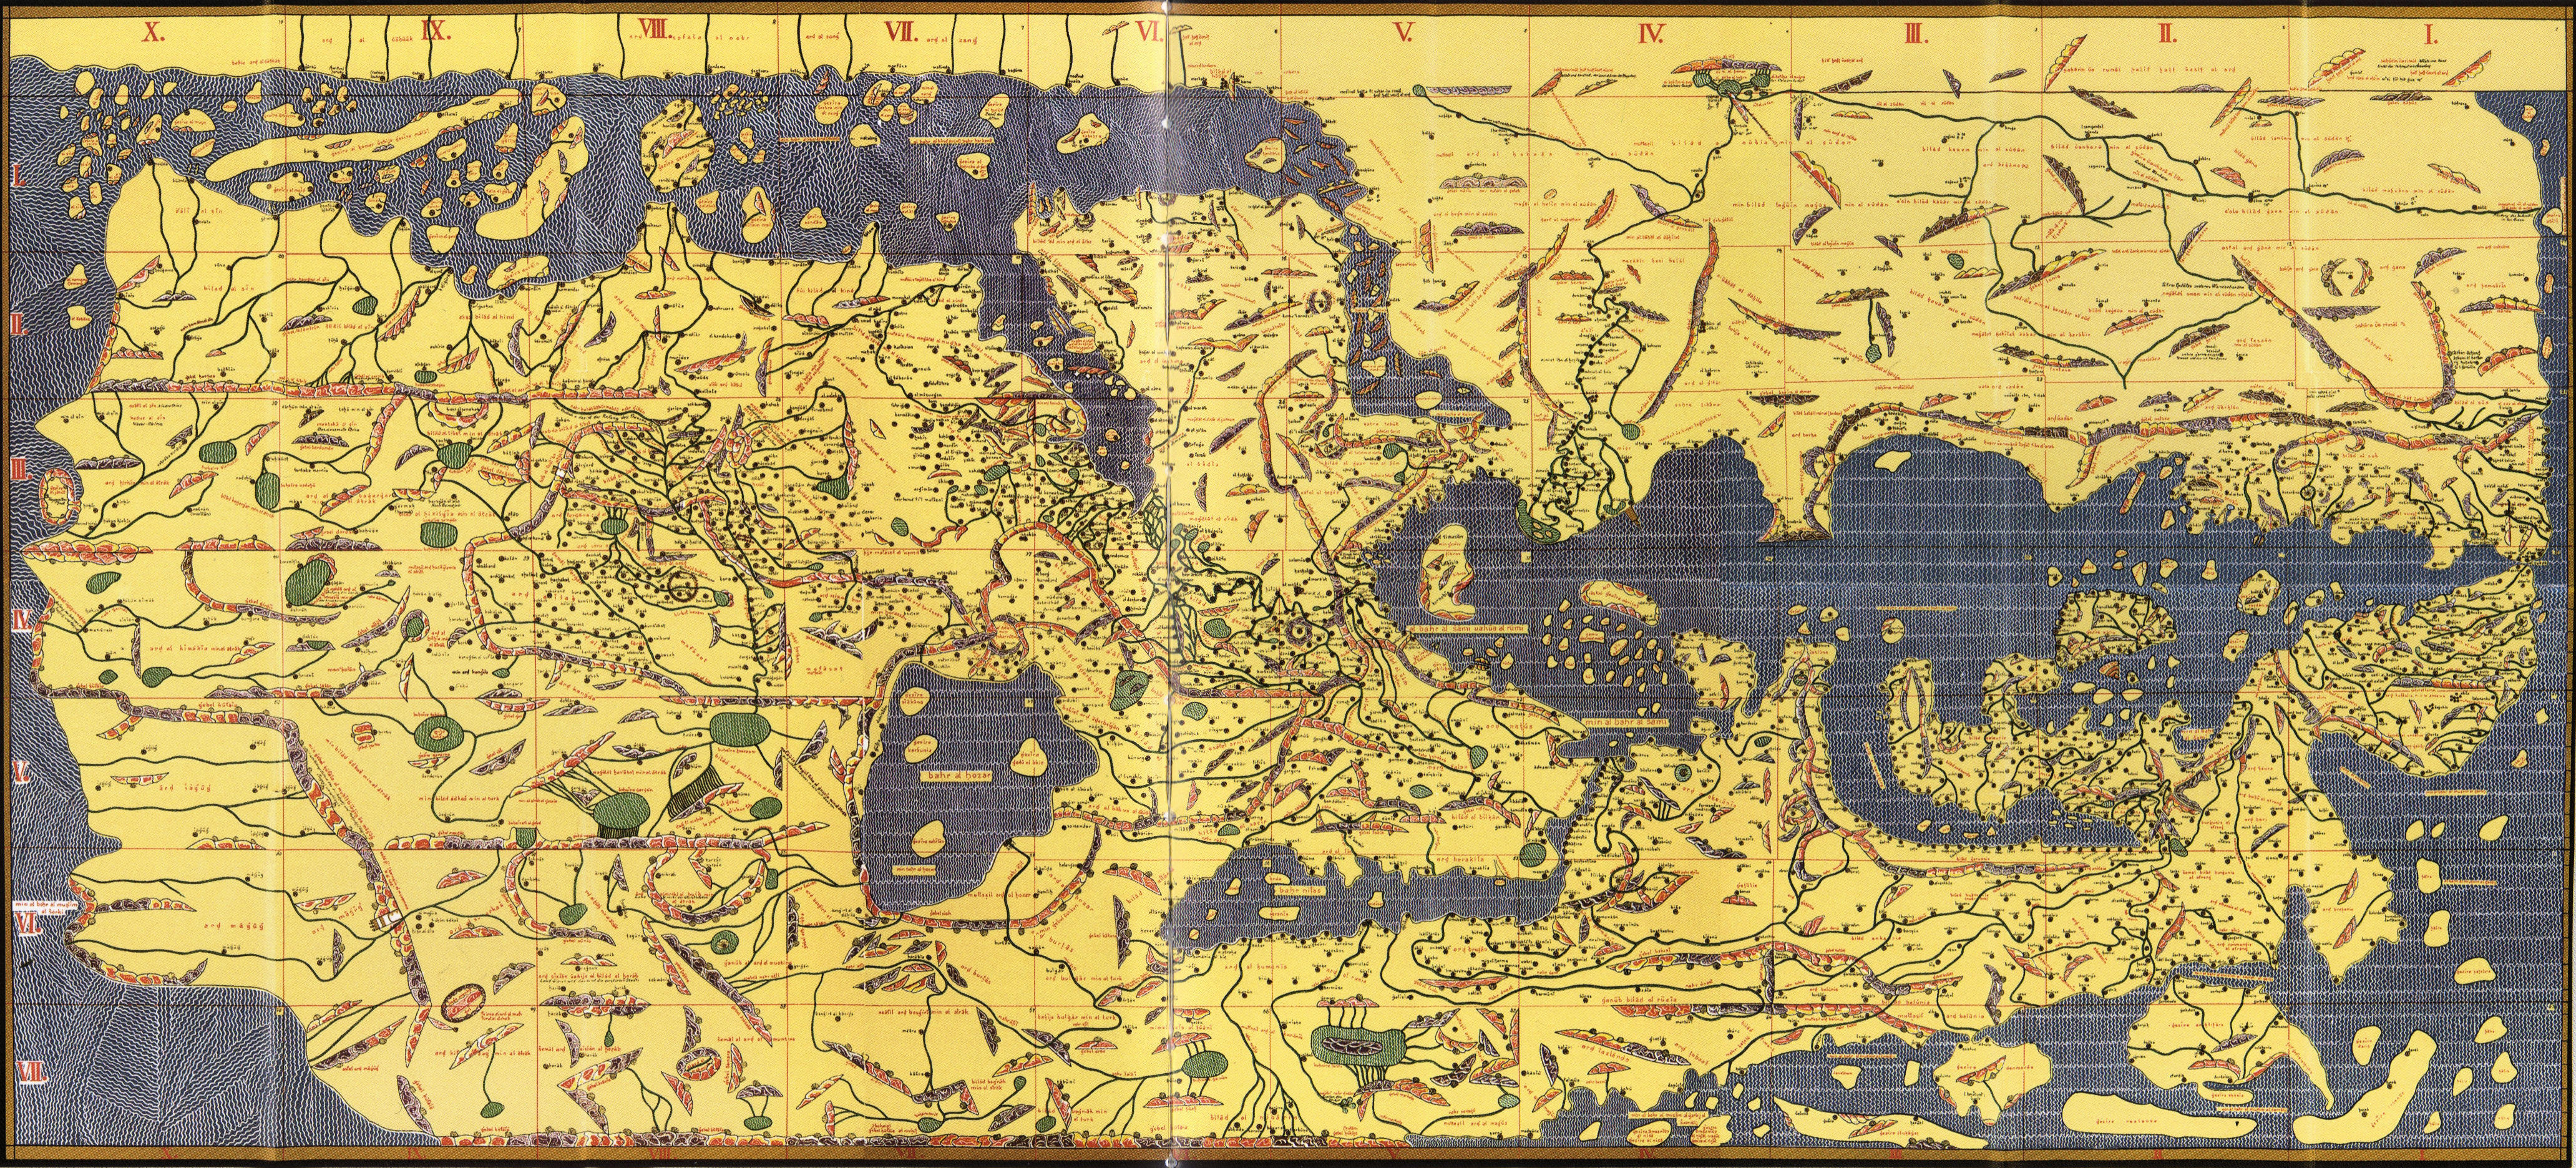
\includegraphics[width=1\textwidth]{figures/TabulaRogeriana.jpg}}
\vskip2pt
\caption{Tabula Rogeriana digambar oleh Al-Idrisi pada tahun 1154 untuk Raja Normandia Roger II dari Sisilia, setelah delapan menetap di istananya, di mana dia bekerja untuk penjelasan dan ilustrasi peta.}
\end{figure}

\section{Penentuan Kordinat}
Kordinat digunakan untuk mengacu sebuah titik lokasi di muka bumi, adapun beberapa jenis standar kordinat yang digunakan adalah.

\subsection{Kordinat Internasional}
Kordinat internasional dikenal dengan long dan lat.


\subsection{Kordinat Indonesia}
Masih ingatkah pelajaran geografi tentang letak Indonesia? maka kita bisa melihat jawaban tersebut dalam kordinat berbahasa indonesia.


%%%%%%%%%%%%%%%%%%%%%%%%%%%%%%%%%%%%%%%%%%%%%%%%%%%%%%
%% optional prologue or prologues
% \chapter{Chapter Title}
% \prologue{<text>}{<author attribution>}

%%%%%%%%%%%%%%%%%%%%%%%%%%%%%%%%%%%%%%%%%%%%%
% Edited Book: Author and Affiliation
%%%%%%%%%%%%%%%%%%%%%%%%%%%%%%%%%%%%%%%%%%%%%

% After \chapter{Chapter Title}, you can
% enter the author name and embed the affiliation with
% \chapterauthors{(author name, or names)
% \chapteraffil{(affiliation or affiliations)}
% }    

% For instance:
% \chapter{Chapter Title}
% \chapterauthors{G. Alvarez and R. K. Watts
% \chapteraffil{Carnegie Mellon University, Pittsburgh, Pennsylvania}

% For separate affiliations you can use \affilmark{(number)} after
% the name of a particular author and before the matching affiliation:

% For instance:
% \chapter{Chapter Title}
% \chapterauthors{George Smeal, Ph.D.\affilmark{1}, Sally Smith,
% M.D.\affilmark{2}, and Stanley Kubrick\affilmark{1}
% \chapteraffil{\affilmark{1}AT\&T Bell Laboratories
% Murray Hill, New Jersey\\
% \affilmark{2}Harvard Medical School,
% Boston, Massachusetts}
% }

%%%%%%%%%%%%%%%%%%%%%%%

%% short version of section head, or one without \\ supplied in sq. brackets.

% \section[Introduction and fugue]{Introduction\\ and fugue}
% \subsection[This is the subsection]{This is the\\ subsection}
% \subsubsection{This is the subsubsection}
% \paragraph{This is the paragraph}

% \begin{chapreferences}{widest label}
% \bibitem{<label>}Reference
% \end{chapreferences}

% optional chapter bibliography using BibTeX,
% must also have \usepackage{chapterbib} before \begin{document}
% Must use root file with \include{chap1}, \include{chap2} form.
%\bibliographystyle{plain}
%\bibliography{<your .bib file name>}

% optional appendix at the end of a chapter:
% \chapappendix{<chap appendix title>}
% \chapappendix{} % no title

%%%%%%%%%%%%%%%%%%%%%%%%%%%%%%%%%%%%%%%%%%%%%%%%%%%%%%%%%%%%%%%%
%% End Matter >>>>>>>>>>>>>>>>>>

% \appendix{<optional title for appendix at end of book>}
% \appendix{} % appendix without title

% \begin{references}{<widest label>}
% \bibitem{sampref}Here is reference.
% \end{references}

%%%%%%%%%%%%%%%%%%%%%%%%%%%%%%%%%%%%%%%%%%%%%%%%%%%%%%%%%%%%%%%%
%% Optional Problem Sets: Can use this at the end of each chapter or at end
%% of book

% \begin{problems}
% \prob
% text

% \prob
% text

% \subprob
% text

% \subprob
% text

% \prob
% text
% \end{problems}

%%%%%%%%%%%%%%%%%%%%%%%%%%%%%%%%%%%%%%%%%%%%%%%%%%%%%%%%%%%%%%%%
%% Optional Exercises: Can use this at the end of each chapter or at end
%% of book

% \begin{exercises}
% \exer
% text

% \exer
% text

% \subexer
% text

% \subexer
% text

% \exer
% text
% \end{exercises}

\bibliographystyle{IEEEtran}
\bibliography{aku}
%%%%%%%%%%%%%%%%%%%%%%%%%%%%%%%%%%%%%%%%%%%%%%%%%%%%%%%%%%%%%%%%
%% INDEX: Use only one index command set:

%% 1) The default LaTeX Index
\printindex

%% 2) For Topic index and Author index:

% \usepackage{multind}
% \makeindex{topic}
% \makeindex{authors}
% \begin{document}
% ...
% add index terms to your book, ie,
% \index{topic}{A term to go to the topic index}
% \index{authors}{Put this author in the author index}

%% (these are Wiley commands)
%\multiprintindex{topic}{Topic index}
%\multiprintindex{authors}{Author index}

\end{document}

%%%%%%% Demo of section head containing sample macro:
%% To get a macro to expand correctly in a section head, with upper and
%% lower case math, put the definition and set the box 
%% before \begin{document}, so that when it appears in the 
%% table of contents it will also work:

\newcommand{\VT}[1]{\ensuremath{{V_{T#1}}}}

%% use a box to expand the macro before we put it into the section head:

\newbox\sectsavebox
\setbox\sectsavebox=\hbox{\boldmath\VT{xyz}}

%%%%%%%%%%%%%%%%% End Demo


Other commands, and notes on usage:

-----
Possible section head levels:
\section{Introduction}
\subsection{This is subsection}
\subsubsection{This is subsubsection}
\paragraph{This is the paragraph}

-----
Tables:
 Remember to use \centering for a small table and to start the table
 with \hline, use \hline underneath the column headers and at the end of 
 the table, i.e.,

\begin{table}[h]
\caption{Small Table}
\centering
\begin{tabular}{ccc}
\hline
one&two&three\\
\hline
C&D&E\\
\hline
\end{tabular}
\end{table}

For a table that expands to the width of the page, write

\begin{table}
\begin{tabular*}{\textwidth}{@{\extracolsep{\fill}}lcc}
\hline
....
\end{tabular*}
%% Sample table notes:
\begin{tablenotes}
$^a$Refs.~19 and 20.

$^b\kappa, \lambda>1$.
\end{tablenotes}
\end{table}

-----
Algorithm.
Maintains same fonts as text (as opposed to verbatim which uses fixed
width fonts). Space at beginning of line will be maintained if you
use \ at beginning of line.

\begin{algorithm}
{\bf state\_transition algorithm} $\{$
\        for each neuron $j\in\{0,1,\ldots,M-1\}$
\        $\{$   
\            calculate the weighted sum $S_j$ using Eq. (6);
\            if ($S_j>t_j$)
\                    $\{$turn ON neuron; $Y_1=+1\}$   
\            else if ($S_j<t_j$)
\                    $\{$turn OFF neuron; $Y_1=-1\}$   
\            else
\                    $\{$no change in neuron state; $y_j$ remains %
unchanged;$\}$ .
\        $\}$   
$\}$   
\end{algorithm}

-----
Sample quote:
\begin{quote}
quotation...
\end{quote}

-----
Listing samples

\begin{enumerate}
\item
This is the first item in the numbered list.

\item
This is the second item in the numbered list.
\end{enumerate}

\begin{itemize}
\item
This is the first item in the itemized list.

\item
This is the first item in the itemized list.
This is the first item in the itemized list.
This is the first item in the itemized list.
\end{itemize}

\begin{itemize}
\item[]
This is the first item in the itemized list.

\item[]
This is the first item in the itemized list.
This is the first item in the itemized list.
This is the first item in the itemized list.
\end{itemize}

%% Index commands
Author and Topic Indices, See docs.pdf and w-bksamp.pdf
